\section{Simulation}

The simulation portion of this assignment was done, as usual, with the assistance of the ngspice software, that allows one to perform detailed analysis of the circuits taught in the lectures.
\par
Starting from the simplified ngspice file provided by the professor, we developed the circuit with the aid of not only the theory presented in the classes, but also the circuit drawn in the presential laboratory class.
 
After building a more complex circuit in this way, we executed time in order to obtain the required measurements such as the impedances and the voltage gain 
\begin{figure}[h] \centering
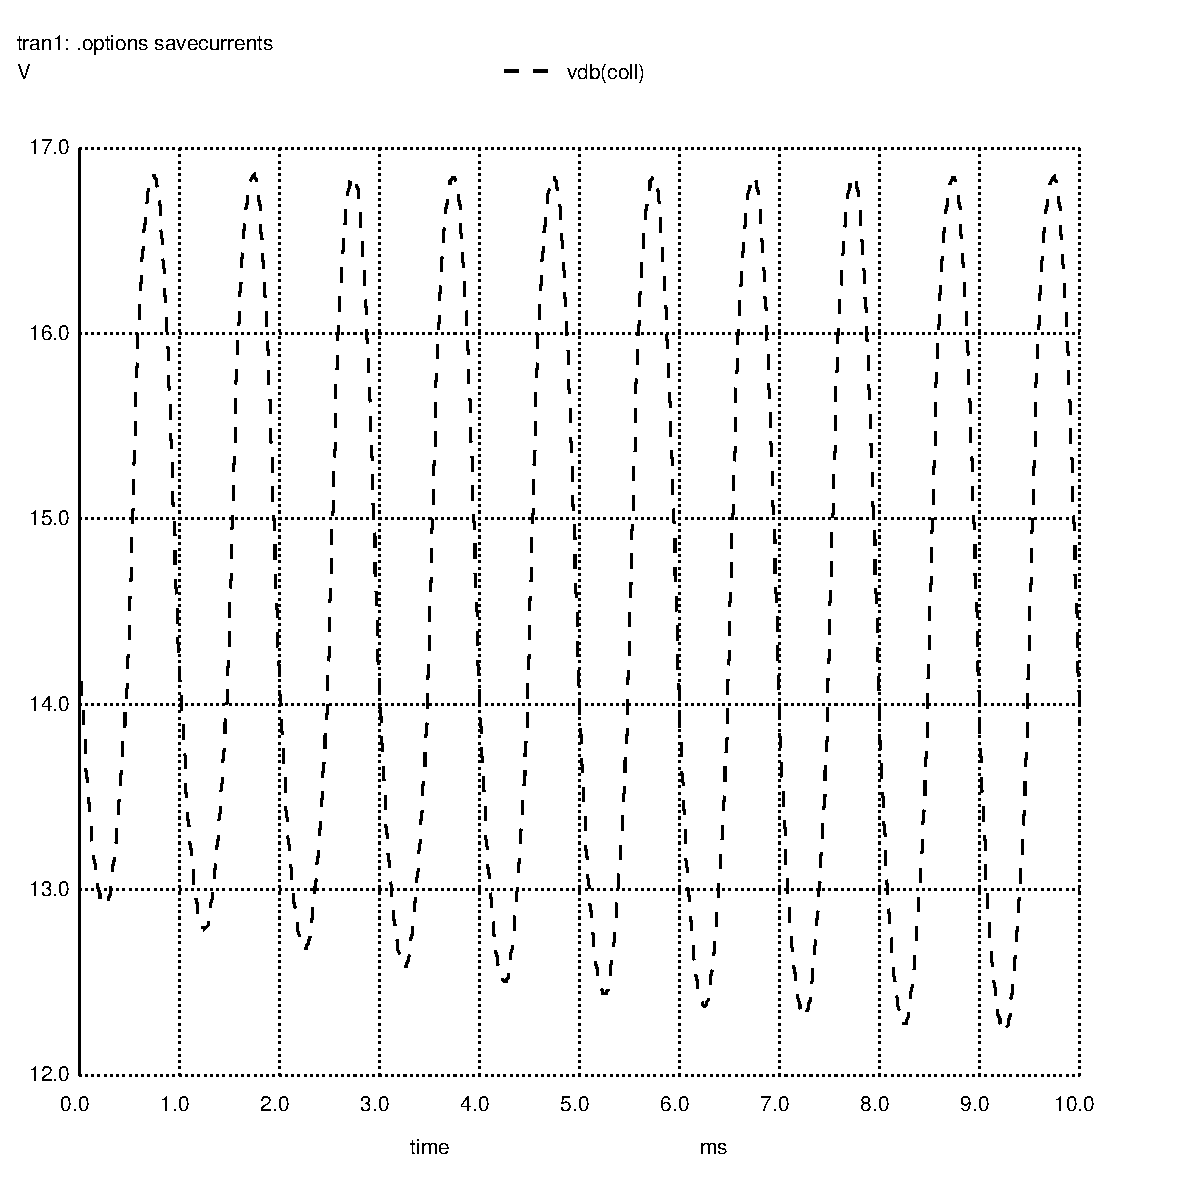
\includegraphics[width=0.8\linewidth]{vo1.eps}
\caption{ Voltage output }
\end{figure}

\begin{figure}[h] \centering
\includegraphics[width=0.8\linewidth]{vo1f.eps}
\caption{ Voltage output, in dB }
\end{figure}

\begin{figure}[h] \centering
\includegraphics[width=0.8\linewidth]{phase.eps}
\caption{ Output phase, in degrees}
\end{figure}

\begin{table}[h]
  \centering
  \begin{tabular}{|l|r|}
    \hline    
    {\bf Parameter} & {\bf Value} \\ \hline
    \input{data_TAB}
  \end{tabular}
  \caption{ Simulation Gain and Impedance }
\end{table}

\begin{table}[h]
  \centering
  \begin{tabular}{|l|r|}
    \hline    
    {\bf Parameter} & {\bf Value} \\ \hline
    \input{imp_out_TAB}
  \end{tabular}
  \caption{ Output impedance  }
\end{table}

\par

Furthermore, a frequency analysis was also carried out so as to obtain the frequency values defining the pass-band, and thus the central frequency value that was relevant to the merit calculation.

\begin{table}[h]
  \centering
  \begin{tabular}{|l|r|}
    \hline    
    {\bf Parameter} & {\bf Value} \\ \hline
    \input{freq_TAB}
  \end{tabular}
  \caption{ Frequency Values }
\end{table}
\par
Finally the parameters that defined the quality of our merit, were also calculated, and are presented in the following table.

\begin{table}[h]
  \centering
  \begin{tabular}{|l|r|}
    \hline    
    {\bf Parameter} & {\bf Value} \\ \hline
    \input{merit_TAB}
  \end{tabular}
  \caption{ Merit defining parameters  }
\end{table}

Furthermore, we modified the values of our circuit parameters (resistors and capacitors) in an exertion to increase our merit figure. These parameters were placed in the introduction.



%tabela

%O q escrevi em cima pode ser dividido depois a medida q se apresentam os plots e tabelas
